\documentclass{article}

\usepackage{pgfplots}

\title{Problem Solving and Modelling Task}
\author{Alexander Arthur}

\begin{document}

\maketitle

\section{Assumptions}
dam is not tidal, no flow in from rivers

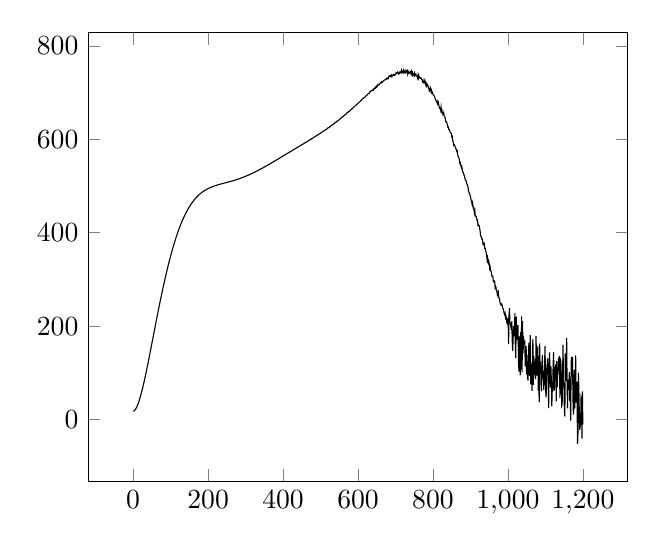
\begin{tikzpicture}
	\begin{axis}
		\addplot[domain=0:1200, samples=1000]{17.8730885286334562067622755421325564384460449218750000000000000000000000000000000000000000000000000000*x^0+0.1120815185722794510292388281413877848535776138305664062500000000000000000000000000000000000000000000*x^1+0.0963702813624544574189201284752925857901573181152343750000000000000000000000000000000000000000000000*x^2+-0.0010369252628716120207680306819497673131991177797317504882812500000000000000000000000000000000000000*x^3+0.0000052120407983112755089557914522924164657524670474231243133544921875000000000000000000000000000000*x^4+-0.0000000151231183341966975223223722344517705451494293811265379190444946289062500000000000000000000000*x^5+0.0000000000271033558930827350391106063374571676950763876590144718647934496402740478515625000000000000*x^6+-0.0000000000000303859693394145203763310252481745569037808671342126842773723183199763298034667968750000*x^7+0.0000000000000000206983539823052845229210332446346277152059031862255111811066399241099134087562561035*x^8+-0.0000000000000000000078183795389526744051833613203930513058234461917569736992984080758972709190857131*x^9+0.0000000000000000000000012543516506984718924958977014763435597845526396834216371694868175958037515016*x^10};
	\end{axis}
\end{tikzpicture}

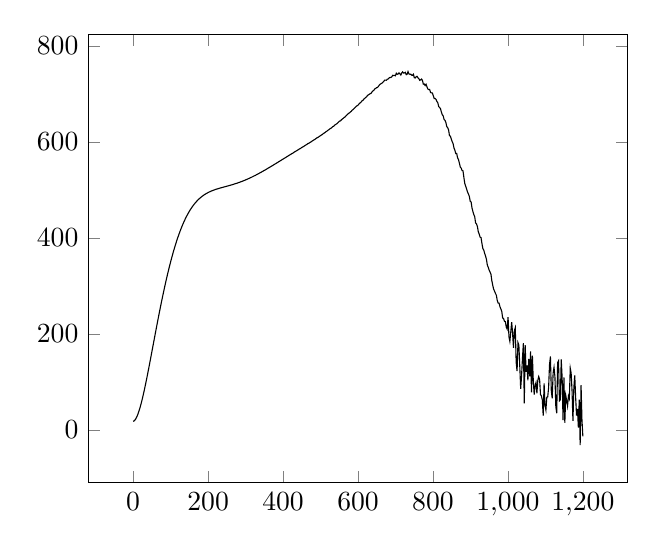
\begin{tikzpicture}
	\begin{axis}
		\addplot[domain=0:1200, samples=500]{17.87308852863345620676227554213255643844604492187500*x^0+0.11208151857227945102923882814138778485357761383057*x^1+0.09637028136245445741892012847529258579015731811523*x^2+-0.00103692526287161202076803068194976731319911777973*x^3+0.00000521204079831127550895579145229241646575246705*x^4+-0.00000001512311833419669752232237223445177054514943*x^5+0.00000000002710335589308273503911060633745716769508*x^6+-0.00000000000003038596933941452037633102524817455690*x^7+0.00000000000000002069835398230528452292103324463463*x^8+-0.00000000000000000000781837953895267440518336132039*x^9+0.00000000000000000000000125435165069847189249589770*x^10};
	\end{axis}
\end{tikzpicture}

\begin{tikzpicture}
	\begin{axis}
		\addplot[domain=0:1200, samples=1000]{17.87308852863345620676*x^0+0.11208151857227945103*x^1+0.09637028136245445742*x^2+-0.00103692526287161202*x^3+0.00000521204079831128*x^4+-0.00000001512311833420*x^5+0.00000000002710335589*x^6+-0.00000000000003038597*x^7+0.00000000000000002070*x^8+-0.00000000000000000001*x^9+0.00000000000000000000*x^10};
	\end{axis}
\end{tikzpicture}

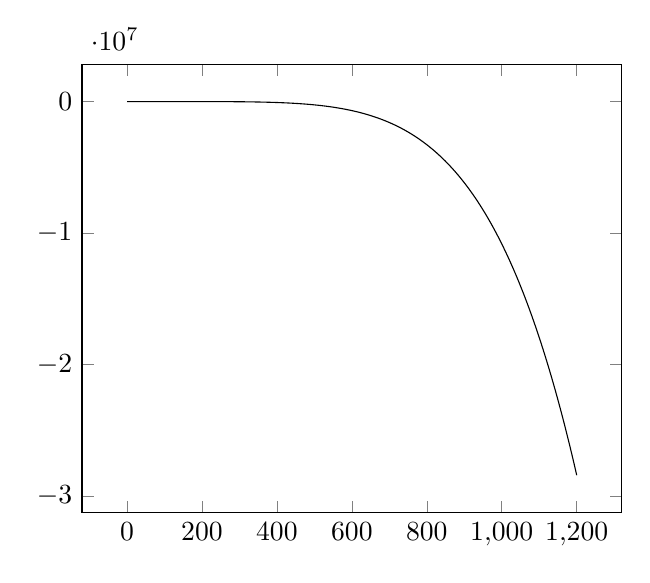
\begin{tikzpicture}
	\begin{axis}
		\addplot[domain=0:1200, samples=1000]{17.8730885286*x^0+0.1120815186*x^1+0.0963702814*x^2+-0.0010369253*x^3+0.0000052120*x^4+-0.0000000151*x^5+0.0000000000*x^6+-0.0000000000*x^7+0.0000000000*x^8+-0.0000000000*x^9+0.0000000000*x^10};
	\end{axis}
\end{tikzpicture}


\end{document}